\chapter{Technische Einzelheiten der Drohne} 
\section{Die Teile}\label{sec:Teile}

Um die für die Drohnenkonstruktion erforderlichen Komponenten zu bestimmen, wurden umfassende Recherchen durchgeführt, mit dem Ziel, geeignete Drohnenteile zu identifizieren und zu beschaffen. Die in der Arbeit verwendete Drohen ist eine FVP-Racing-Drohen\cite{FPV} im Quadkopter\cite{Quadkopter} Art, jedoch ohne Videobrille und Kamera. 

Im Rahmen dieser Untersuchung wurden die folgenden Teile als relevant eingestuft und anschliessend beschafft. Im Anhang ist eine \hyperref[ch:infoteile]{Tabelle} der Teile mit den wichtigsten Funktion und Eigenschaft zu finden.

\subsection{Akkumulator} \label{sec:Akku} 
Für den Quadkopter wurde eine Batterie des Herstellers OVONIC verwendet. Die Batterie weist eine Spannung von 22,2 Volt auf und ein Gewicht von 222 Gramm. Ihre Funktion besteht in der kontinuierlichen und stabilen Spannungsversorgung sämtlicher elektronischer Komponenten der Drohne. Sie ist für Racing-Drohnen optimiert und gewährleistet so eine besondere Leistungsfähigkeit. Die verwendete Lithium-Polymer (LiPo)-Technologie ist aufgrund ihres vorteilhaften Energie-zu-Gewicht-Verhältnisses für den Einsatz in Drohnen prädestiniert.\cite{Akku} Der Akkumulator besteht aus sechs identischen Zellen. Es gäbe auch kleinere Akkumulatoren, die aus vier Zellen bestehen. Aufgrund der leistungsstarken Motoren, die verbaut wurden, fiel die Entscheidung zugunsten des Systems, das mit sechs Zellen betrieben wird.

\subsection{Motoren}\label{sec:Motoren}

Die Motoren einer Drohne sind von essenzieller Bedeutung für das Abheben und die Steuerung. Mittels einer variierenden Drehrichtung, die sich in ihrer Drehzahl unterscheiden kann, ist eine Bewegung der Drohne in alle Richtungen sowie eine Rotation um die eigene Achse möglich. Für die Konstruktion wurden vier bürstenlose Motoren ausgewählt, die mit 5-Zoll-Propellern kompatibel sind. Diese Motoren sind ebenfalls für Racing-Drohnen geeignet und weisen ein Gewicht von jeweils 30 Gramm auf. \cite{Motorenkauf} Die bürstenlose Bauweise erhöht die Effizienz und Lebensdauer der Motoren. Die Kommutierung erfolgt elektronisch durch einen Controller, der die Phasen der Statorwicklungen zur optimalen Zeit schaltet, um ein kontinuierliches Drehmoment zu erzeugen. \cite{Motorenstudy} Diese präzise Steuerung ermöglicht eine gleichmässige Rotation des Motors sowie eine exakte Leistungsabgabe. Bürstenlose Motoren zeichnen sich durch ein optimales Leistungs-Gewicht-Verhältnis aus, was sie insbesondere für den Einsatz in Racing-Drohnen prädestiniert.


\subsection{Propeller}\label{sec:Propeller} 
\begin{wrapfigure}{r}{0.3\textwidth}  % r für rechts, 0.3\textwidth für Bildbreite
	\centering
	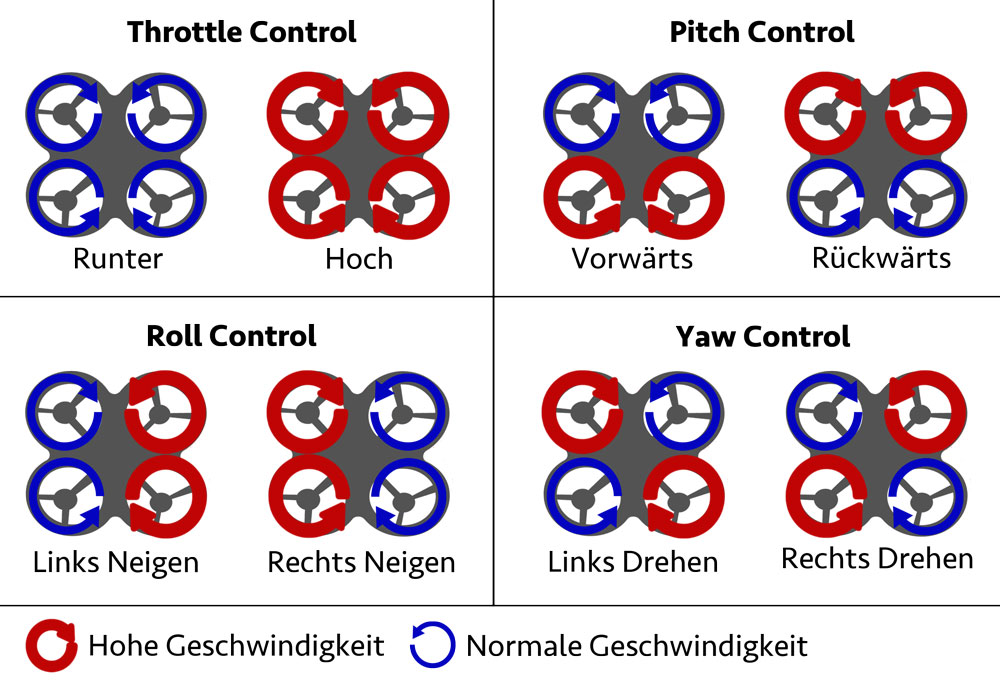
\includegraphics[width=0.28\textwidth]{MotionDE.jpg} % Passt die Bildbreite an
	\caption{Die Grundlagen der Drohnensteuerung}
	\label{fig:motionde}
\end{wrapfigure}
Die für den Flug der Drohne verantwortlichen Propeller erzeugen durch ihre Drehbewegung Schub, der für die Aufrechterhaltung der Flugposition in der Luft erforderlich ist. Die aerodynamische Form der Propellerblätter optimiert die Luftströmung, sodass diese effizient bewegt wird. Bei einem Quadkopter drehen die Propeller über Kreuz jeweils in die gleiche Richtung, was eine unkontrollierte Rotation der Drohne um die Z-Achse verhindert. Dieses Prinzip findet ebenfalls Anwendung bei der gezielten Rotation der Drohne, wie bei \autoref{fig:motionde} gezeigt.

\subsection{Speedy Bee F7 V3 Stack}  \label{sec:F7V3}
Der Flight Controller (FC) stellt das Herzstück der Drohne dar und basiert auf einem leistungsstarken STM32F7-Mikrocontroller. Dieser bietet ausreichend Rechenleistung für die Bewältigung komplexer Steueraufgaben sowie die Verarbeitung von Sensordaten, Steuerbefehlen und Flugalgorithmen. \cite{Stack}

Der Electronic Speed Controller (ESC), der direkt unter dem FC verbaut wurde, regelt die elektrische Leistung von der Batterie zu den Motoren. Die vom FC vorgegeben Motordrehzahl werden durch den ESC praktisch umgesetzt. Der für das Projekt eingebaute Speedy Bee F7 V3 Stack vereint eine Vielzahl von Funktionen in einem Gerät und ist mit einer Vielzahl anderer Komponenten kompatibel. Erwähnenswert sind auch die Sensoren wie die \hyperref[sec:IMU]{IMU} und der \hyperref[sec:Barometer]{Barometer}. Diese befinden sich ebenfalls direkt auf der Platine des Speedy Bee F7 V3 Stacks und werden später noch detaillierter beschrieben.

\subsection{ELRS-Empfänger} \label{sec:ELRS-Empfänger}
Der Express Long Range System (ELRS)-Empfänger \cite{ELRS} fungiert als Antenne der Drohne. Er empfängt Steuerbefehle über eine Frequenz von 2.4 Gigaherz und bietet den Vorteil einer stabilen Verbindung über grössere Entfernungen. Der ELRS-Empfänger wandelt die Radiofrequenzsignale in elektrische Impulse um, die vom FC in Steuerbefehle für den ESC umgesetzt werden. Auf diese Weise wird ein Signal erzeugt, wenn an der Fernbedienung ein Stick bewegt wird.

\subsection{Fernbedienung}  
Die RadioMaster Boxer ist eine vielseitige und moderne Funkfernbedienung, die speziell für den Einsatz mit Drohnen und anderen ferngesteuerten Modellen entwickelt wurde. Mit einem Frequenzbereich von 2,4 Gigaherz ermöglicht sie eine stabile Verbindung zwischen Sender und Empfänger\cite{RadioController}. Sie unterstützt bis zu 16 Kanäle, was eine präzise Steuerung selbst bei komplexen Anforderungen sicherstellt \cite{RadioController}. Ein besonderes Merkmal ist die Auswahl zwischen zwei internen Hochfrequenzmodulen: einem ExpressLRS (ELRS)-Modul\footnote{ExpressLRS (ELRS) ist ein modernes, Open-Source-Funkübertragungssystem, das speziell für ferngesteuerte Modelle wie Drohnen und RC-Fahrzeuge (Remote controlle Fahrzeuge) entwickelt wurde. Es bietet eine extrem geringe Latenz(Verzögerung) von nur 4–8 ms, eine hohe Reichweite von mehreren Kilometern und eine robuste Signalübertragung dank der LoRa-Modulationstechnologie (LoRa = Long Range). ExpressLRS unterstützt Frequenzbänder wie 2,4 Gigaherz für schnelle Reaktionen und 900 MHz für maximale Reichweite. Durch seine Flexibilität, Anpassungsfähigkeit und Kompatibilität mit verschiedenen Geräten ist ELRS ideal für FPV-Racing, Long-Range-Flüge sowie industrielle Anwendungen. Zudem zeichnet es sich durch geringen Stromverbrauch und eine aktive Entwickler-Community aus.} und einem 4-in-1/CC2500 Multi-Protokoll-Modul, wodurch eine breite Kompatibilität mit verschiedenen Empfängern gewährleistet wird \cite{ATOMRC}.

Die technische Ausstattung der RadioMaster Boxer umfasst einen leistungsstarken STM32\-F407VGT6-Prozessor mit 1 MB Flash-Speicher und 192 KB RAM, der eine schnelle und zuverlässige Signalverarbeitung ermöglicht. Vorinstalliert ist die Open-Source-Firmware EdgeTX, die durch ihre Flexibilität und Anpassbarkeit überzeugt. %Zusätzlich ist die Fernbedienung ergonomisch gestaltet und mit hochwertigen Hall-Gimbals \footnote{Hall-Gimbals sind Steuerknüppel, die mit Hall-Sensoren arbeiten, um Bewegungen präzise und berührungslos zu messen. Die Position des Hebels wird dabei durch Veränderungen im Magnetfeld erfasst, ohne dass es zu mechanischem Verschleiss kommt, wie er bei herkömmlichen Potentiometern zu beobachten ist. Ihre Langlebigkeit, das sanfte Steuergefühl und die Möglichkeit der individuellen Anpassung von Härte und Selbstzentrierung sind signifikante Vorteile. Hall-Gimbals finden vor allem in Fernbedienung für Drohnen oder RC-Geräte Anwendung, wo Präzision und Zuverlässigkeit von entscheidender Bedeutung sind.} ausgestattet, die eine präzise Steuerung und ein komfortables Benutzererlebnis bieten. 
Die Energieversorgung kann wahlweise über eine 7,4V 2-Zellen Lithium-Polymer-Batterie oder zwei 3,7V 18650 Lithium-Ionen-Zellen erfolgen, wodurch eine flexible und zuverlässige Nutzung sichergestellt wird.\cite{RadioController}\cite{ATOMRC}

Im Kontext der Drohnennsteuerung nimmt die Wahl der Fernbedienung eine entscheidende Rolle ein. Funkfernbedienung, wie die RadioMaster Boxer, senden Signale an die Drohne, um diese in Bezug auf Richtung, Höhe und Geschwindigkeit zu steuern. Die Drohne empfängt diese Signale und setzt sie um, indem sie die Motoren entsprechend ansteuert \cite{Steuerung}. Dafür ist es essenziell, dass sowohl die Fernbedienung als auch der Empfänger dieselbe Sprache sprechen, also dass sie das gleiche Kommunikationsprotokoll verwenden – in diesem Fall ExpressLRS. % Die Steuerung wird durch Gyroskope und Flugsteuerungssysteme ergänzt, die Daten von Sensoren verarbeiten und die Stabilität der Drohne in der Luft gewährleisten. Diese Systeme sind von entscheidender Bedeutung, um automatisierte Bewegungen, präzise Manöver und Stabilisierung auch bei Störungen wie Wind oder Turbulenzen sicherzustellen \cite{Steuerung}.

Die Zuverlässigkeit und Präzision der Funkverbindung sind dabei von entscheidender Bedeutung, da Störungen in der Funkverbindung potenziell gefährliche Situationen verursachen könnten. Hochwertige Fernbedienungen wie die RadioMaster Boxer sind daher sehr wichtig\cite{Steuerung}. Ihre Vielseitigkeit und Leistungsfähigkeit machen sie zu einer idealen Wahl für die anspruchsvolle Steuerung von Drohnen in wissenschaftlichen und technischen Projekten.


\subsection{Smoke Stopper} \label{sec:Smoke Stopper}
Der Smoke Stopper\cite{SmokeStopper} ist ein Kurzschlussschutz, der bei einem Kurzschluss, also dem ungewollten Kontakt zweier nicht verbundener Leitungen (0 Ohm), eingreift und den Stromkreis unterbricht. Der Smoke Stopper wurde in diesem Fall zur Absicherung der Drohne im Falle einer fehlerhaften Lötstelle eingesetzt.\footnote{Das Projekt verlief planmässig, sodass der Smoke Stopper nicht aktiv wurde.}

\subsection{Kondensator} \label{sec:Kondensator}
Ein Kondensator ist ein elektronisches Bauteil, das in zahlreichen Geräten Anwendung findet. Er speichert elektrische Energie kurzzeitig und gleicht dadurch Schwankungen im Stromfluss aus. Dies schützt die Bauteile im Stromkreis vor Spannungsspitzen und sorgt gleichzeitig für einen gleichmässigeren Stromfluss, was zu einer stabileren und zuverlässigeren Leistung führt. Ein passender Kondensator war dem Flight Controller bereits beigelegt und in diesem Projekt verwendet. 

\subsection{Frame}   \label{sec:Frame}
Der Frame \cite{Frame} stellt die Struktur, das Gestell der Drohne dar, an dem alle Komponenten befestigt werden. Der Rahmen besteht aus Kohlefaser, einem leichten, aber robusten Material. Der Rahmen ist im Deadcat-Design\cite{fpv24deadcatframes} konzipiert, was bedeutet, dass die Motoren in einem diagonalen Layout angeordnet sind, wobei die vorderen und hinteren Arme weiter voneinander entfernt sind als die seitlichen Arme. Dieses Design verbessert das Sichtfeld der FPV-Kamera und reduziert die Störung durch Propeller im Kamerabild. Wichtig war, dass der Frame sowohl leicht als auch robust war, was er eindeutig erfüllt.

\section{Die Sensoren}\label{sec:Sensoren}

Die Integration von Sensoren in die Konstruktion einer Drohne ermöglicht die Schaffung eines komplexen Systemes, das als "Gehirn" der Drohne bezeichnet werden kann. 
Die Funktionalität ermöglicht präzises Fliegen, automatische Funktionen und verbessert die Steuerung sowie die intelligenten Fähigkeiten der Drohne, sich selbst zu regulieren und steuern. 

\subsection{IMU}  \label{sec:IMU}
Die Interial Measurement Unit (IMU) fungiert als Beschleunigungsmesser im Flugcontroller. Sie misst, wie schnell und in welche Richtung sich die Drohne dreht. Dank der IMU ist die Drohne stets in der Lage, ihre Ausrichtung während des Flugs präzise zu bestimmen und entsprechend zu korrigieren, um stabil zu fliegen. Die IMU kann als das innere Gleichgewichtsorgan betrachtet werden, das die Drohne auf Kurs hält, vergleichbar mit dem Innenohr des Menschen. Es besteht aus einem Beschleunigungssensor und einem Gyroskop, das die lineare Beschleunigung sowie die Winkelgeschwindigkeit der Drohne in drei Raumrichtungen (x, y, z) misst. Der Beschleunigungssensor misst die lineare Beschleunigung und der durch die Gravitation verursachten Beschleunigung. Er erfasst Änderungen in der Geschwindigkeit (also Beschleunigungen) und kann durch Integration dieser Messwerte die Geschwindigkeit berechnen. Meistens wird ein kapazitiver\footnote{Ein kapazitiver Drucksensor verwendet zwei parallel angeordnete Platten, von denen eine fest und die andere druckempfindlich ist. Wenn Druck auf die bewegliche Platte ausgeübt wird, verändert sich der Abstand zwischen den Platten und damit die Kapazität des Systems. Diese Kapazitätsänderung wird in ein elektrisches Signal umgewandelt. Kapazitive Drucksensoren zeichnen sich durch hohe Genauigkeit und Langzeitstabilität aus und werden daher in medizinischen und sicherheitskritischen Anwendungen bevorzugt eingesetzt.\cite{Capacitive_vs_Piezoresistive}} oder piezoresistiver\footnote{Ein piezoresistiver Drucksensor arbeitet, indem er die Widerstandsänderung eines Materials misst, wenn Druck auf eine Siliziummembran ausgeübt wird. Auf dieser Membran befinden sich vier Widerstände, die sich verformen, sobald Druck ausgeübt wird, was zu einer Änderung des elektrischen Widerstands führt. Diese Veränderung wird durch eine Wheatstone-Brücke in ein elektrisches Signal umgewandelt.\cite{Capacitive_vs_Piezoresistive} Piezoresistive Drucksensoren sind aufgrund ihrer geringen Produktionskosten weit verbreitet und finden Anwendung in der Automobilindustrie, in Haushaltsgeräten und in Konsumgütern.} Beschleunigungssensor eingesetzt. Das Gyroskop hingegen misst die Winkelgeschwindigkeit um die drei Achsen. Häufig kommt ein MEMS-Gyroskop (Micro-Electro-Mechanical-Systems) zum Einsatz, das auf dem Coriolis-Effekt basiert. 	Dabei detektiert das Gyroskop Rotationsbewegungen, indem es die durch die Rotation erzeugten Corioliskräfte auf winzige, bewegliche Strukturen innerhalb des Sensors misst. Diese Kräfte werden in elektrische Signale umgewandelt, die die Winkelgeschwindigkeit in den drei Raumrichtungen präzise erfassen."\footnote{Die Corioliskraft ist die Kraft, die durch die Rotation der Erde um ihre eigene Achse erzeugt wird. Auf der Nordhalbkugel werden die Teilchen nach rechts und auf der Südhalbkugel nach links abgelenkt. Hurrikane oder der Wasserabfluss drehen auf der Nordhälfte der Erde andersherum als auf der Südhälfte. \cite{Coriolis}} Durch die Kombination der Daten von Beschleunigungssensor und Gyroskop kann die exakte Orientierung der Drohne im Raum ermittelt werden. Dies geschieht, indem die Daten durch ein Kalman-Filter\footnote{Der Kalman-Filter ist ein mathematisches Verfahren zur Schätzung von Systemzuständen, die nicht direkt messbar sind, auf der Grundlage fehlerhafter Beobachtungen. Er kombiniert in jedem Schritt neue Messungen mit bisherigen Schätzungen, um den Fehler zu minimieren. Besonders ist, dass der Filter neben den Schätzwerten auch die Unsicherheiten und Korrelationen zwischen den Schätzfehlern berücksichtigt. Dadurch kann er dynamische Grössen wie Position und Geschwindigkeit präzise schätzen. Der Kalman-Filter wird in vielen technischen Bereichen eingesetzt, etwa zur Positionsbestimmung oder in elektronischen Steuerungssystemen. \cite{Kalman}} verarbeitet werden, um eine optimale Schätzung des Zustands der Drohne zu erhalten. Diese IMU-Daten bilden die Grundlage für die Regelung der Fluglage und zur Stabilisierung der Drohne.

\subsection{Barometer}  \label{sec:Barometer}
Das Barometer misst den Luftdruck, was für eine Drohne in bestimmten Gebieten von enormer Relevanz sein kann, da die Höhe über dem Boden möglichst genau ermittelt werden muss. Dies ist beispielsweise im „Altitude-Hold“-Modus wichtig, bei dem die Drohne automatisch ihre Höhe beibehält. In dieser Maturaarbeit spielt das Barometer ebenfalls eine zentrale Rolle, da es die Berechnung der Sinkgeschwindigkeit im Falle eines Fail-Safes ermöglicht. Diese Anpassung des Fail-Safe-Modus ist ein wesentlicher Bestandteil der vorliegenden Arbeit. Meist wird das Barometer zusätzlich durch ein GPS ergänzt, das ebenfalls die Höhe über dem Meeresspiegel misst. Diese Kombination ermöglicht eine deutlich höhere Genauigkeit. In diesem Fall muss jedoch auf ein GPS verzichtet werden, da der Flight Controller (FC) kein integriertes GPS besitzt und aus Komplexitätsgründen bewusst auf ein externes GPS verzichtet wurde.